% Appendix — remaining fixed-time-budget convergence plots.
% Main text highlights 4 of the 28 cells (Fig.~\ref{fig:exp_time}):
%   two_stops/SX, tollgate/SX (MetaDrive), vshape/shuffle (Scenic),
%   sustained_steer/CSXS (MetaDrive). The 24 remaining cells appear here,
%   one figure per specification (six scenarios each).

Figures~\ref{fig:app_time_two_stop}--\ref{fig:app_time_sustained} show the
convergence of the compositional and monolithic estimates under a fixed time
budget for the remaining 24 specification--scenario cells, complementing the
four highlighted in Fig.~\ref{fig:exp_time}. The two estimates agree within
their confidence intervals across all cells, with the same qualitative
behavior as in the highlighted plots.

\begin{figure}[p]
    \centering
    \captionsetup[subfloat]{justification=centering}
  \subfloat[S$\to$X$\to$S (MetaDrive)]{%
       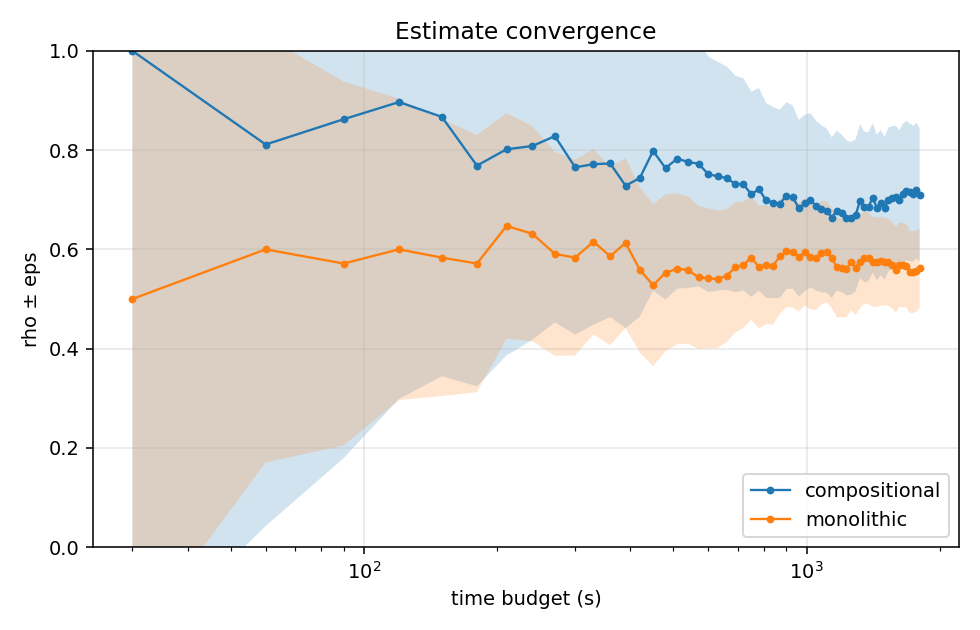
\includegraphics[width=0.49\linewidth,height=100pt,keepaspectratio]{figures/time-budget/metadrive__two_stops__SXS.png}}
    \hfill%
  \subfloat[S$\to$O$\to$C (MetaDrive)]{%
       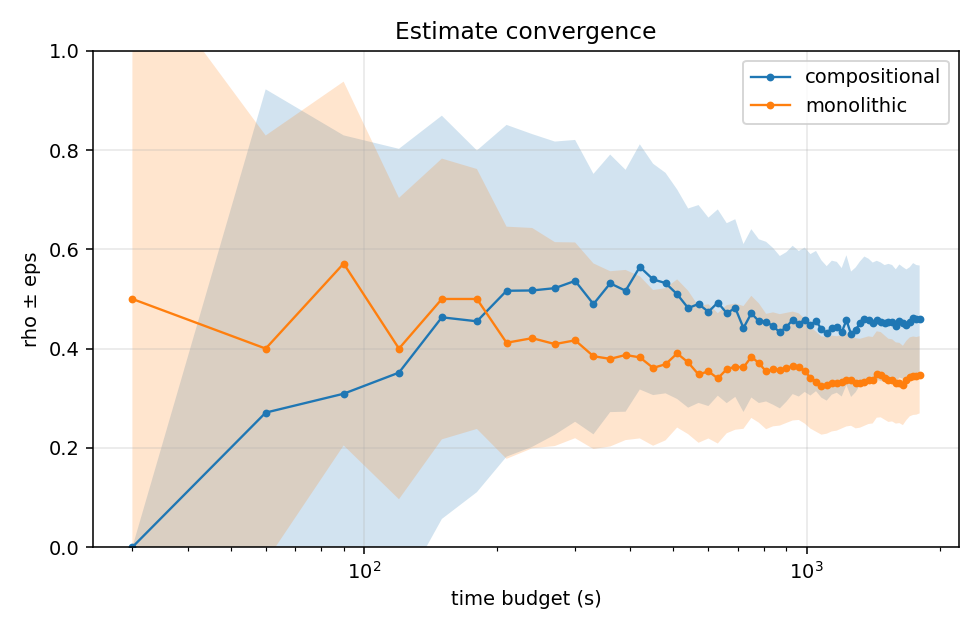
\includegraphics[width=0.49\linewidth,height=100pt,keepaspectratio]{figures/time-budget/metadrive__two_stops__SOC.png}}
\\
  \subfloat[C$\to$S$\to$X$\to$S (MetaDrive)]{%
       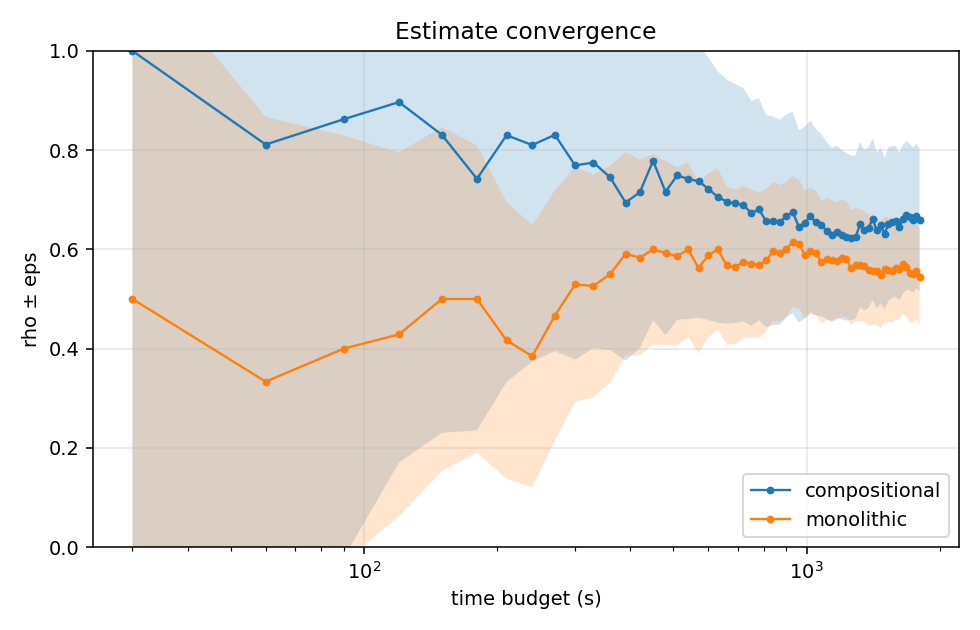
\includegraphics[width=0.49\linewidth,height=100pt,keepaspectratio]{figures/time-budget/metadrive__two_stops__CSXS.png}}
    \hfill%
  \subfloat[C$\to$X$\to$S$\to$X$\to$C (MetaDrive)]{%
       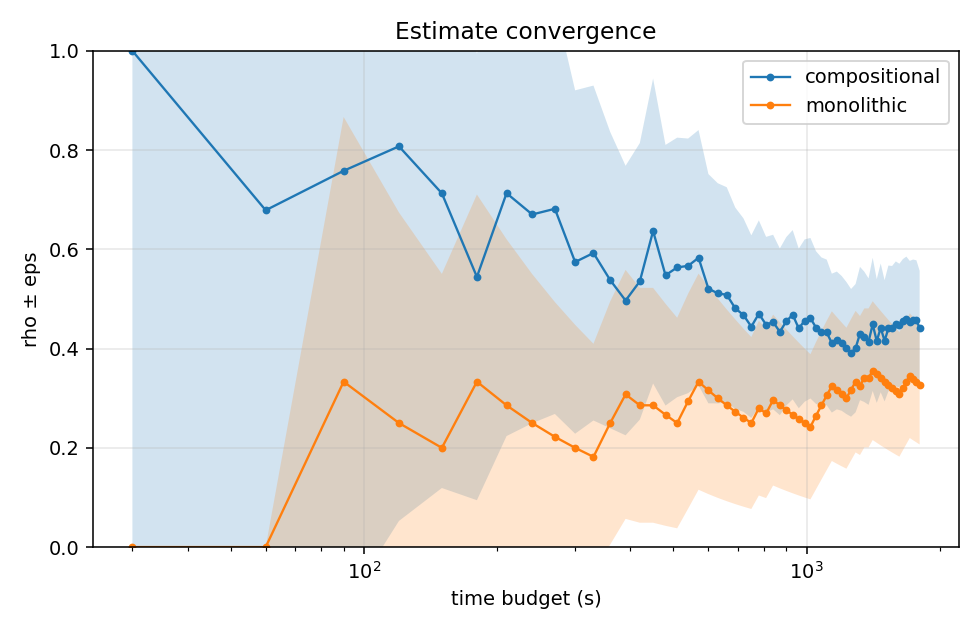
\includegraphics[width=0.49\linewidth,height=100pt,keepaspectratio]{figures/time-budget/metadrive__two_stops__CXSXC.png}}
\\
  \subfloat[S\,$\to$\,choose(C,X,O) (Scenic)]{%
       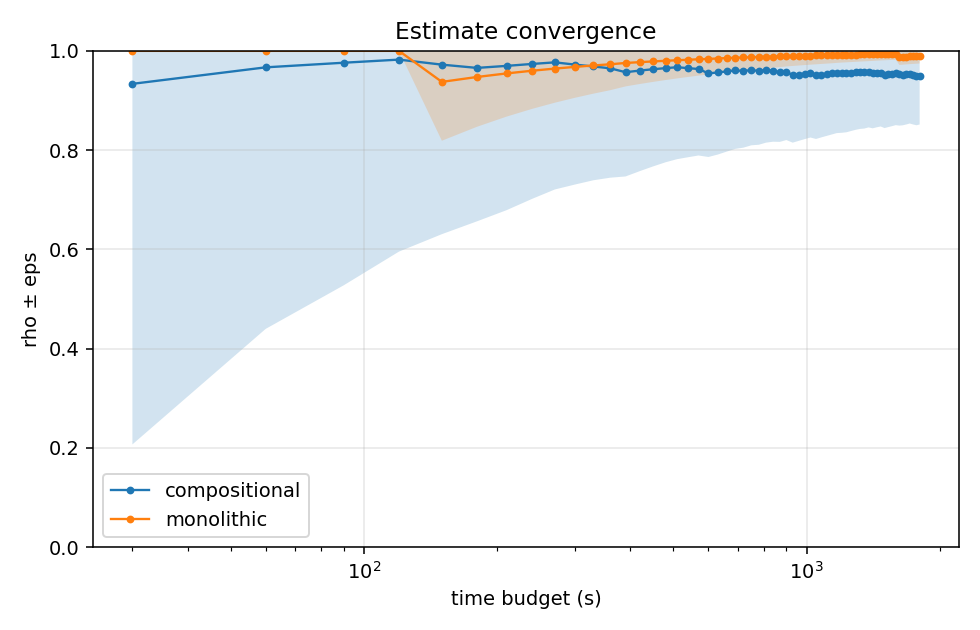
\includegraphics[width=0.49\linewidth,height=100pt,keepaspectratio]{figures/time-budget/scenic__two_stops__choose.png}}
    \hfill%
  \subfloat[S\,$\to$\,shuffle(C,X,O) (Scenic)]{%
       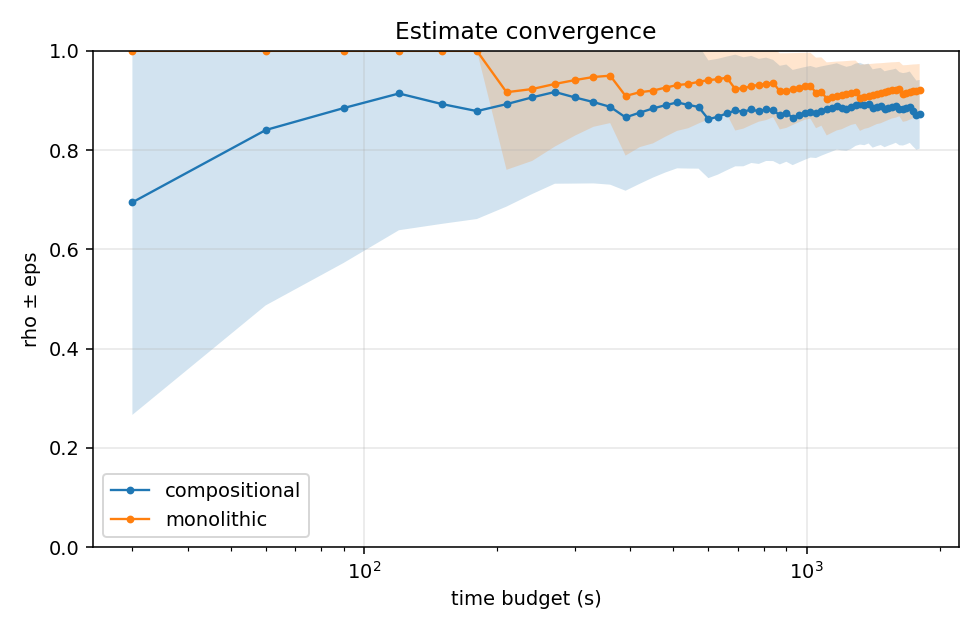
\includegraphics[width=0.49\linewidth,height=100pt,keepaspectratio]{figures/time-budget/scenic__two_stops__shuffle.png}}
  \caption{Fixed-time-budget results for \emph{2-Stop} on the remaining six scenarios.}
  \label{fig:app_time_two_stop}
\end{figure}

\begin{figure}[p]
    \centering
    \captionsetup[subfloat]{justification=centering}
  \subfloat[S$\to$X$\to$S (MetaDrive)]{%
       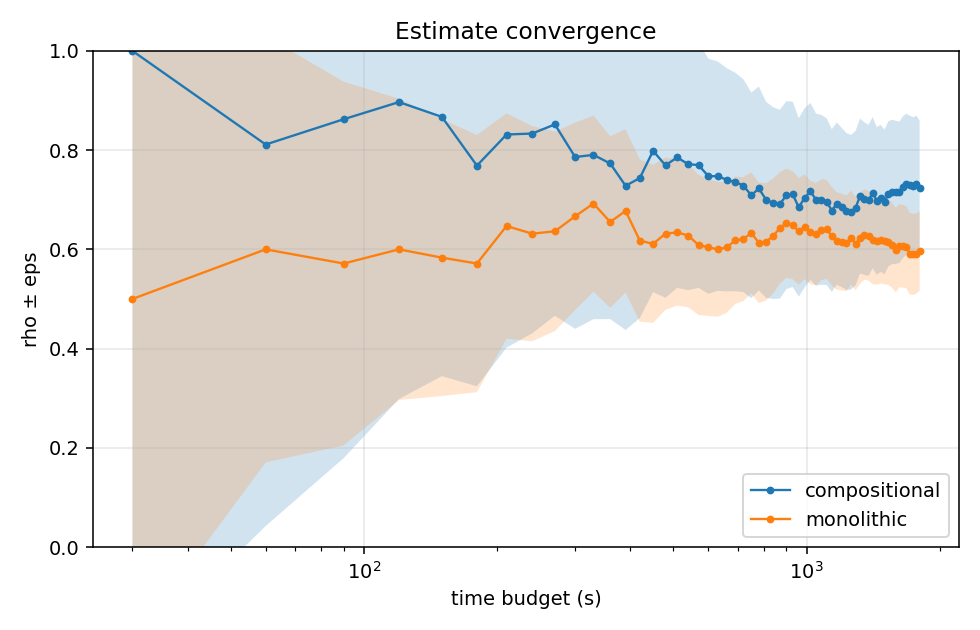
\includegraphics[width=0.49\linewidth,height=100pt,keepaspectratio]{figures/time-budget/metadrive__tollgate__SXS.png}}
    \hfill%
  \subfloat[S$\to$O$\to$C (MetaDrive)]{%
       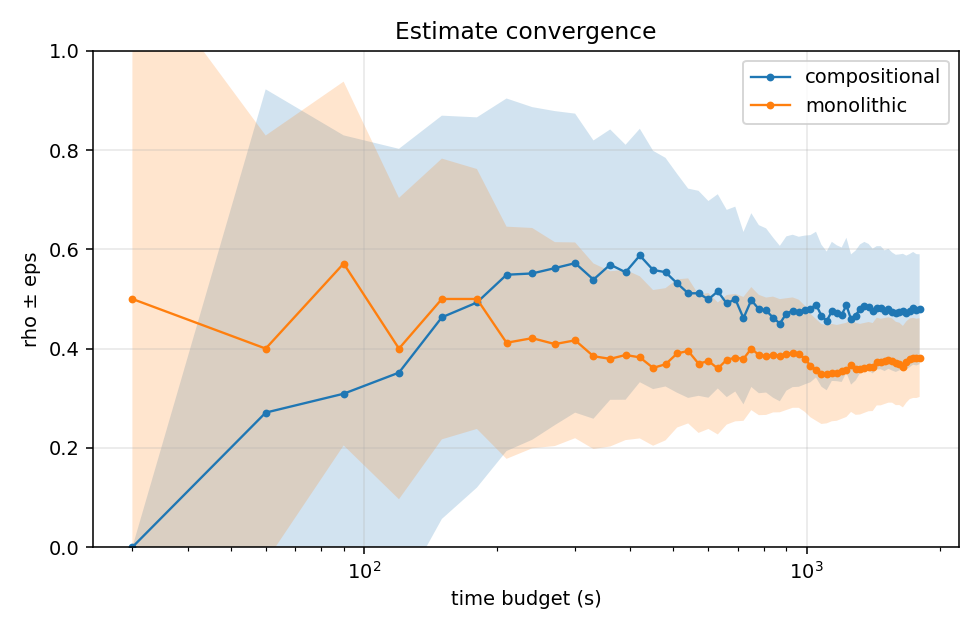
\includegraphics[width=0.49\linewidth,height=100pt,keepaspectratio]{figures/time-budget/metadrive__tollgate__SOC.png}}
\\
  \subfloat[C$\to$S$\to$X$\to$S (MetaDrive)]{%
       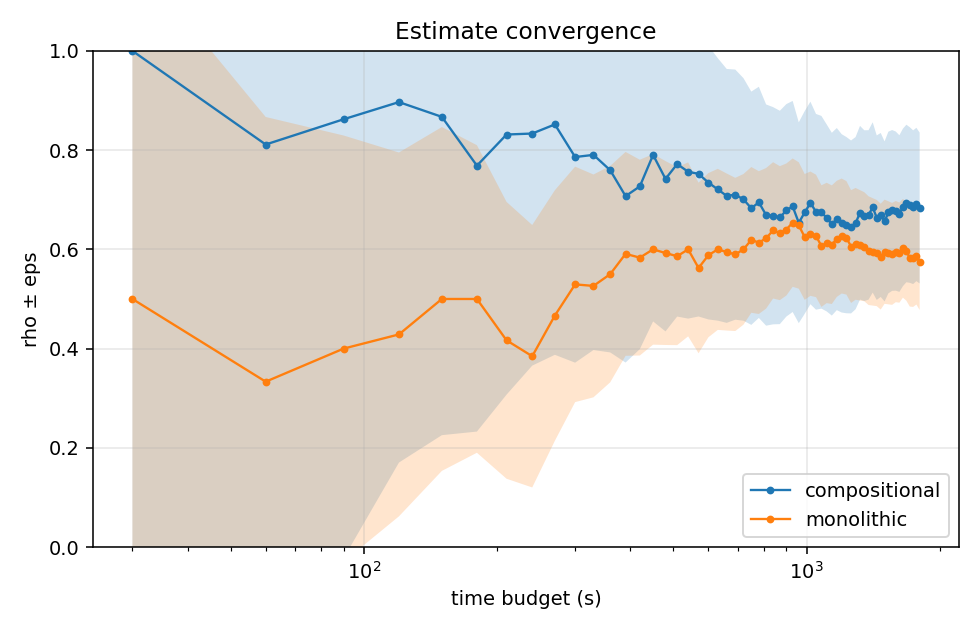
\includegraphics[width=0.49\linewidth,height=100pt,keepaspectratio]{figures/time-budget/metadrive__tollgate__CSXS.png}}
    \hfill%
  \subfloat[C$\to$X$\to$S$\to$X$\to$C (MetaDrive)]{%
       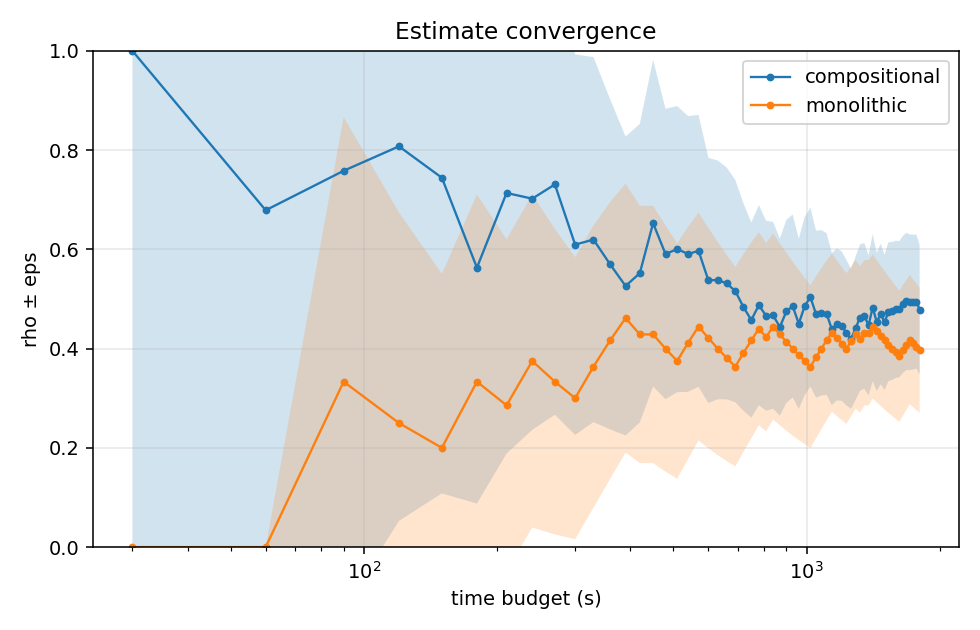
\includegraphics[width=0.49\linewidth,height=100pt,keepaspectratio]{figures/time-budget/metadrive__tollgate__CXSXC.png}}
\\
  \subfloat[S\,$\to$\,choose(C,X,O) (Scenic)]{%
       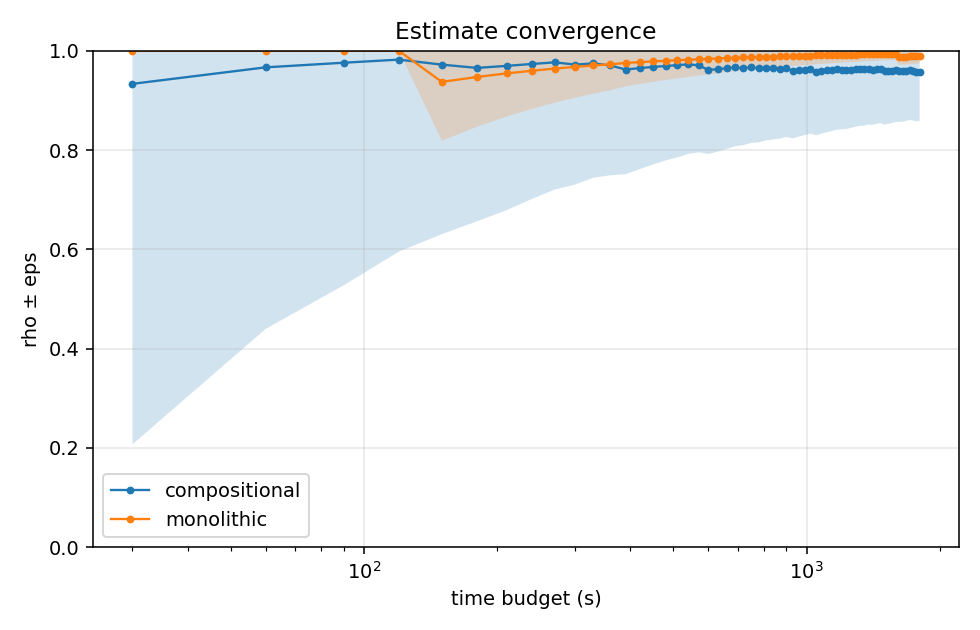
\includegraphics[width=0.49\linewidth,height=100pt,keepaspectratio]{figures/time-budget/scenic__tollgate__choose.png}}
    \hfill%
  \subfloat[S\,$\to$\,shuffle(C,X,O) (Scenic)]{%
       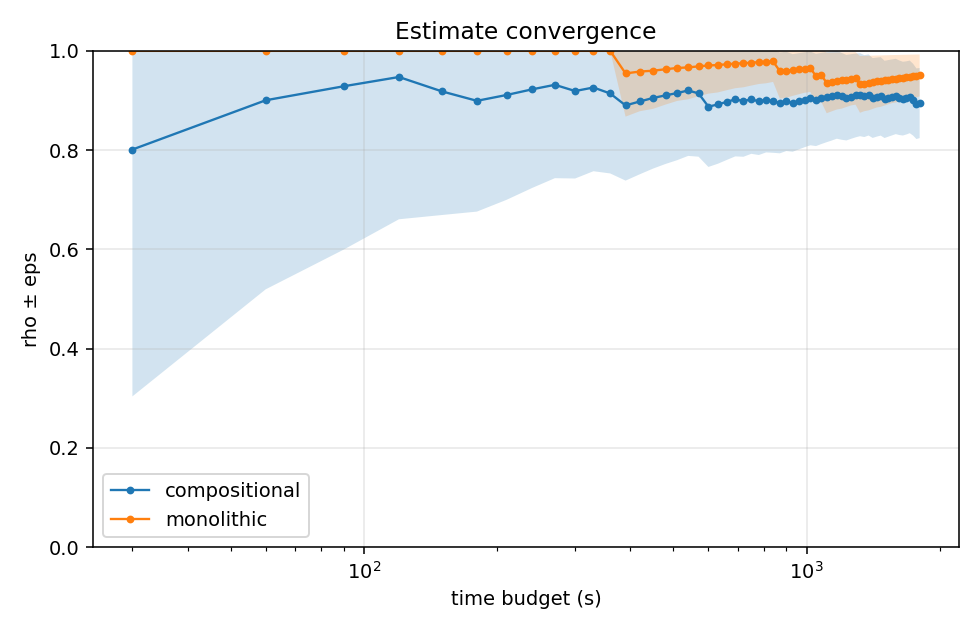
\includegraphics[width=0.49\linewidth,height=100pt,keepaspectratio]{figures/time-budget/scenic__tollgate__shuffle.png}}
  \caption{Fixed-time-budget results for \emph{Tollgate} on the remaining six scenarios.}
  \label{fig:app_time_tollgate}
\end{figure}

\begin{figure}[p]
    \centering
    \captionsetup[subfloat]{justification=centering}
  \subfloat[S$\to$X (MetaDrive)]{%
       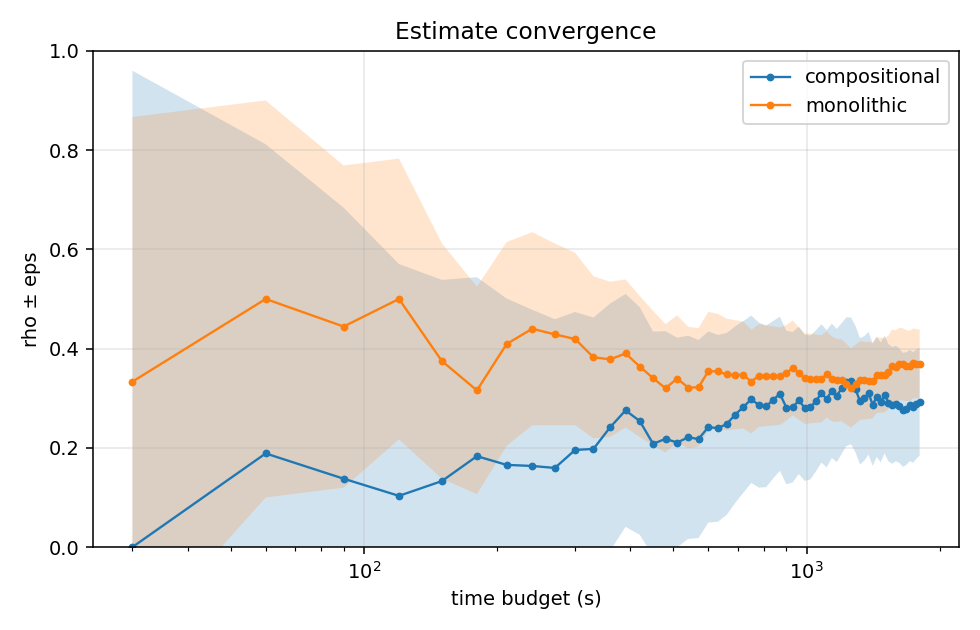
\includegraphics[width=0.49\linewidth,height=100pt,keepaspectratio]{figures/time-budget/metadrive__vshape__SX.png}}
    \hfill%
  \subfloat[S$\to$X$\to$S (MetaDrive)]{%
       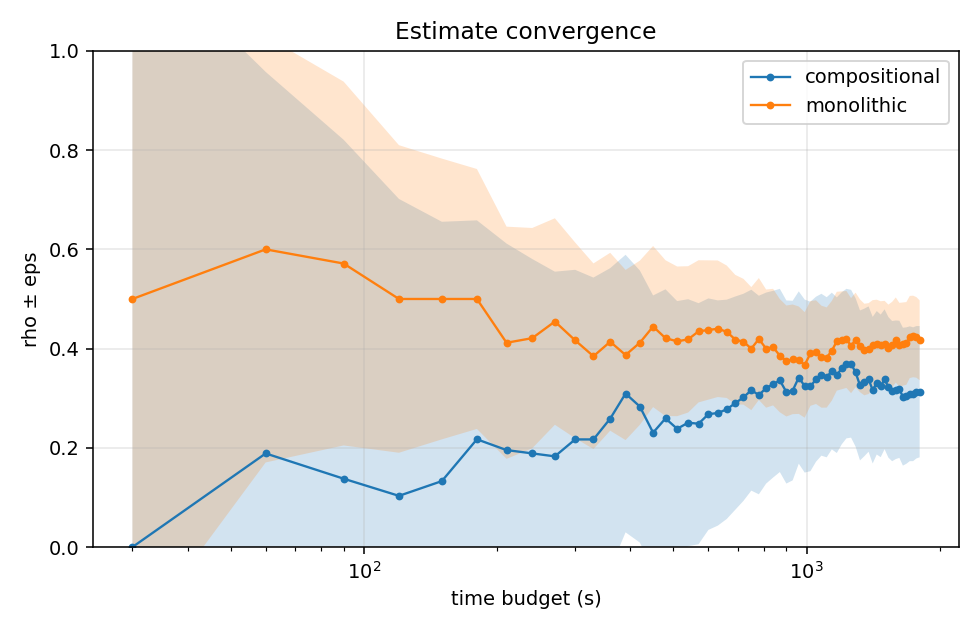
\includegraphics[width=0.49\linewidth,height=100pt,keepaspectratio]{figures/time-budget/metadrive__vshape__SXS.png}}
\\
  \subfloat[S$\to$O$\to$C (MetaDrive)]{%
       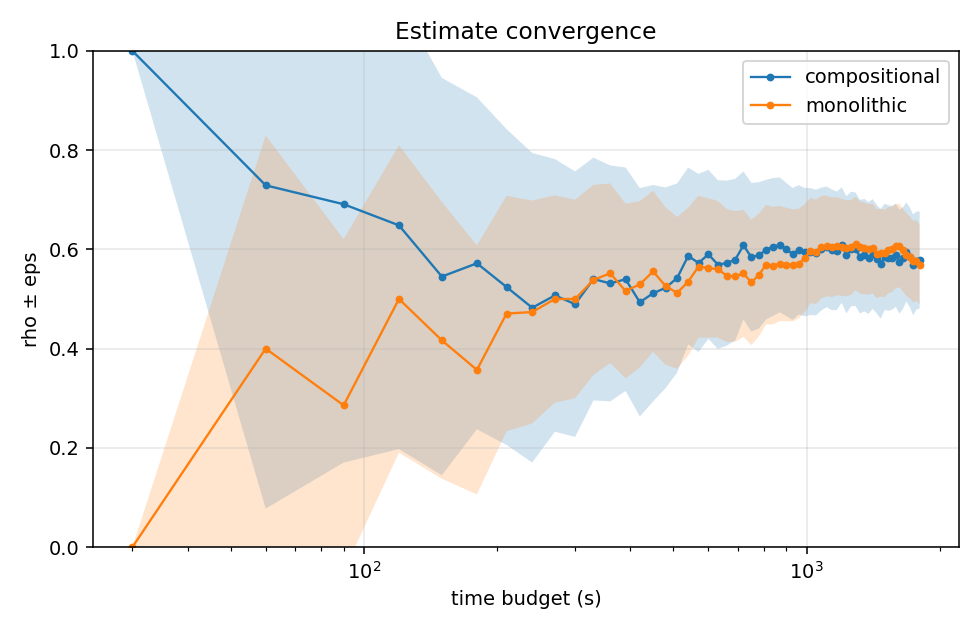
\includegraphics[width=0.49\linewidth,height=100pt,keepaspectratio]{figures/time-budget/metadrive__vshape__SOC.png}}
    \hfill%
  \subfloat[C$\to$S$\to$X$\to$S (MetaDrive)]{%
       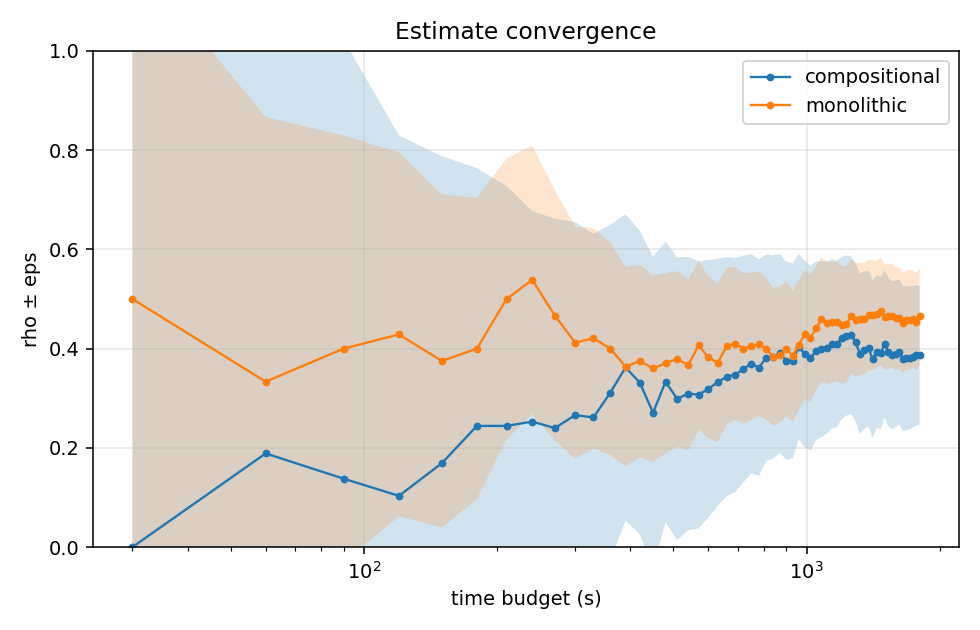
\includegraphics[width=0.49\linewidth,height=100pt,keepaspectratio]{figures/time-budget/metadrive__vshape__CSXS.png}}
\\
  \subfloat[C$\to$X$\to$S$\to$X$\to$C (MetaDrive)]{%
       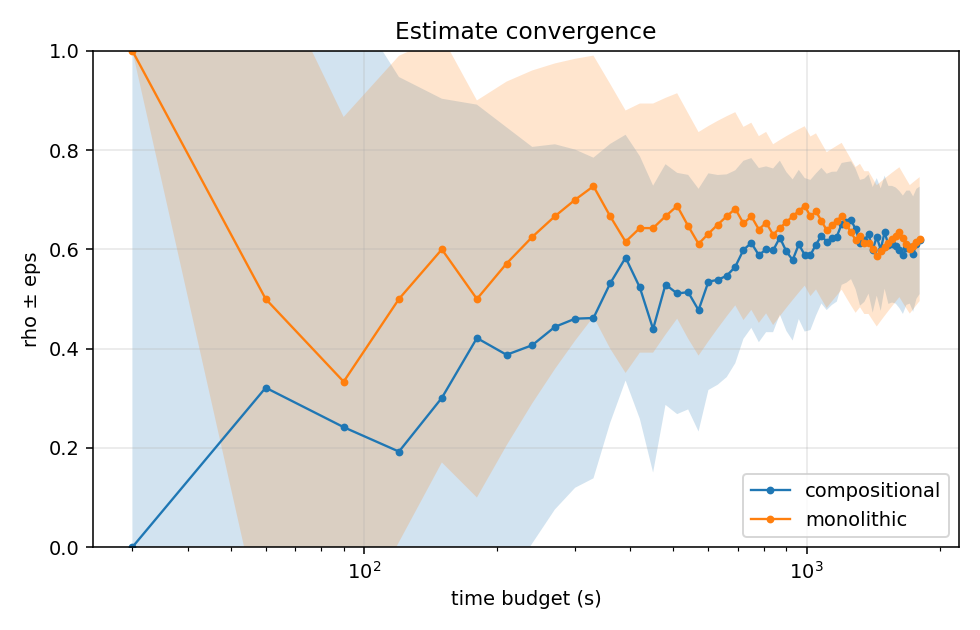
\includegraphics[width=0.49\linewidth,height=100pt,keepaspectratio]{figures/time-budget/metadrive__vshape__CXSXC.png}}
    \hfill%
  \subfloat[S\,$\to$\,choose(C,X,O) (Scenic)]{%
       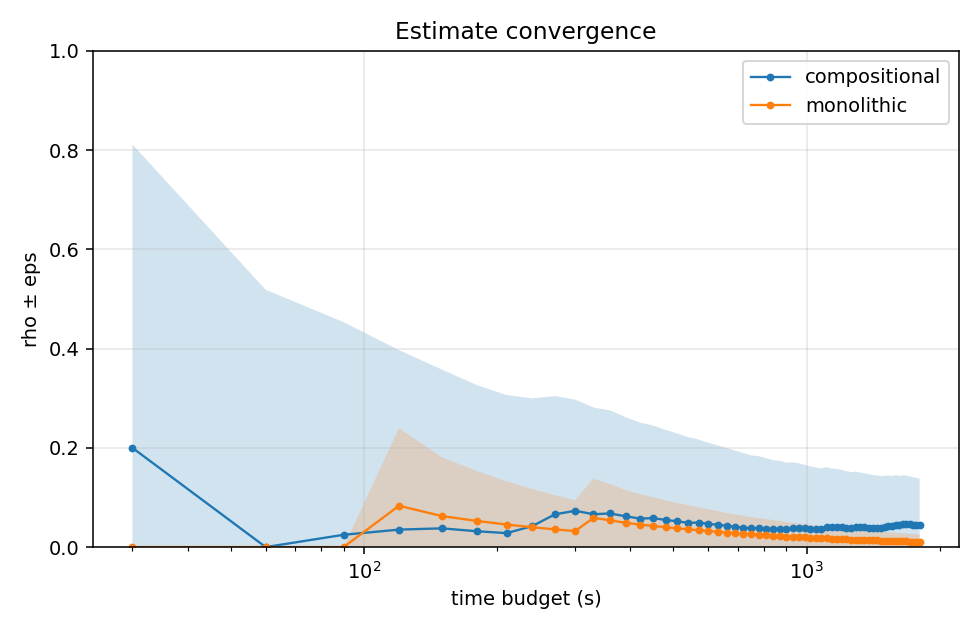
\includegraphics[width=0.49\linewidth,height=100pt,keepaspectratio]{figures/time-budget/scenic__vshape__choose.png}}
  \caption{Fixed-time-budget results for \emph{V-Shaped} on the remaining six scenarios.}
  \label{fig:app_time_v_shaped}
\end{figure}

\begin{figure}[p]
    \centering
    \captionsetup[subfloat]{justification=centering}
  \subfloat[S$\to$X (MetaDrive)]{%
       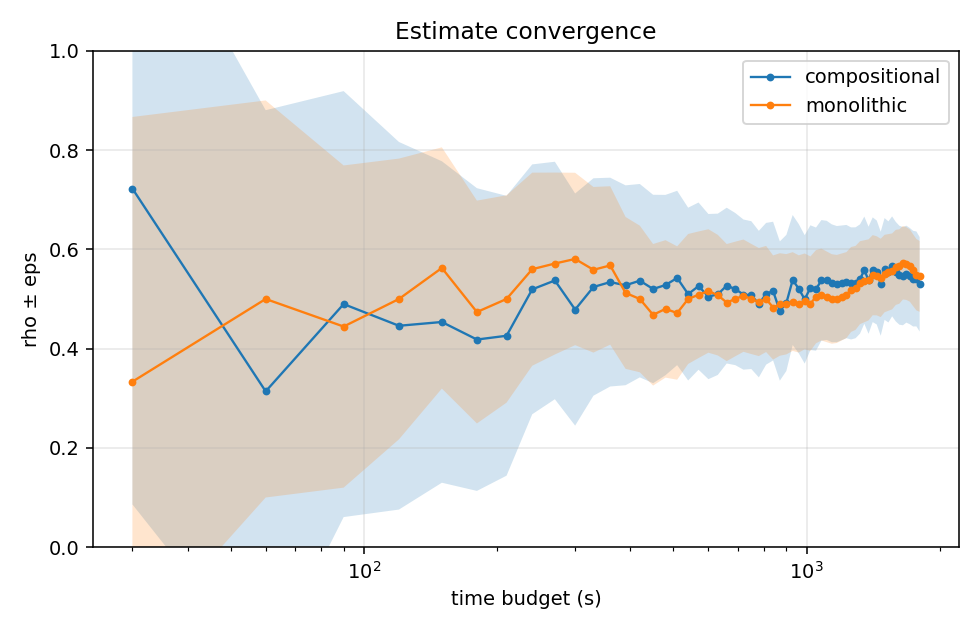
\includegraphics[width=0.49\linewidth,height=100pt,keepaspectratio]{figures/time-budget/metadrive__sustained_steer__SX.png}}
    \hfill%
  \subfloat[S$\to$X$\to$S (MetaDrive)]{%
       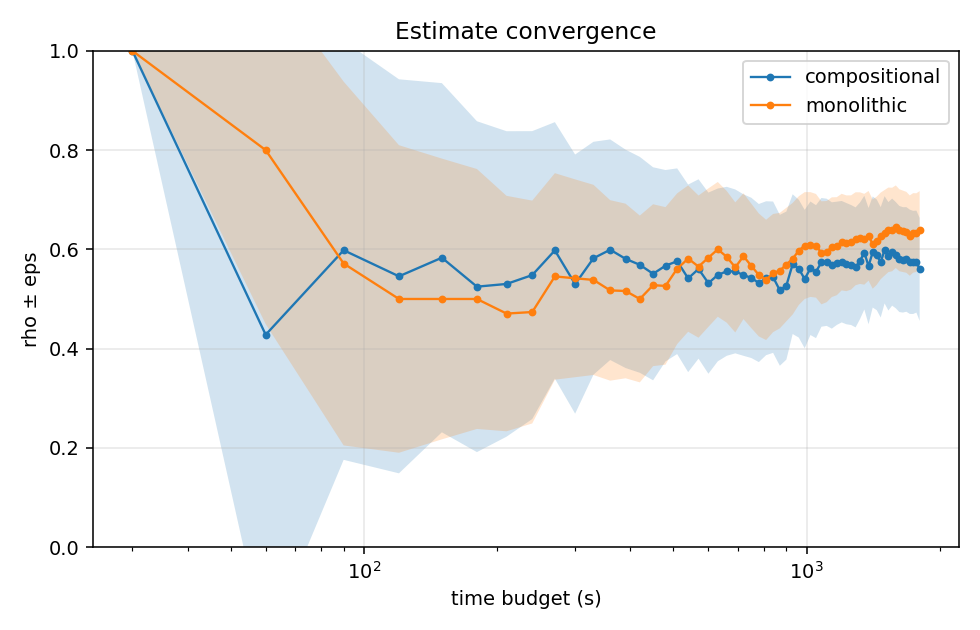
\includegraphics[width=0.49\linewidth,height=100pt,keepaspectratio]{figures/time-budget/metadrive__sustained_steer__SXS.png}}
\\
  \subfloat[S$\to$O$\to$C (MetaDrive)]{%
       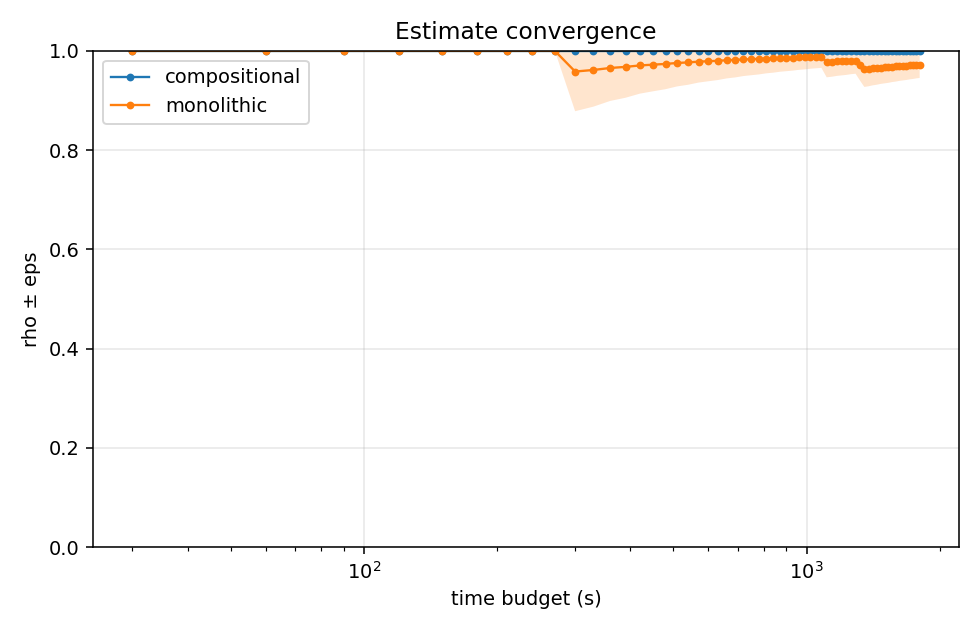
\includegraphics[width=0.49\linewidth,height=100pt,keepaspectratio]{figures/time-budget/metadrive__sustained_steer__SOC.png}}
    \hfill%
  \subfloat[C$\to$X$\to$S$\to$X$\to$C (MetaDrive)]{%
       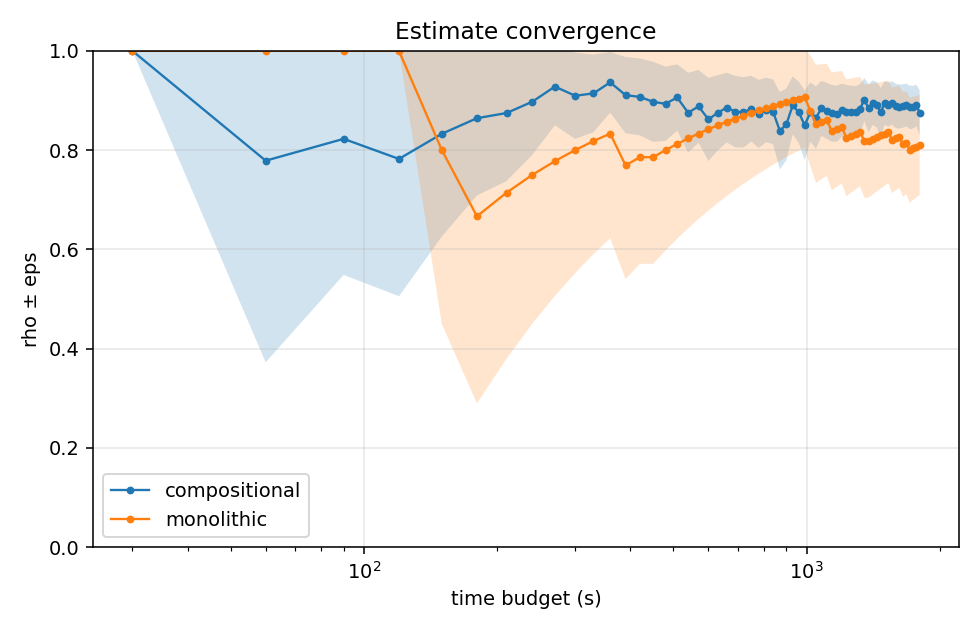
\includegraphics[width=0.49\linewidth,height=100pt,keepaspectratio]{figures/time-budget/metadrive__sustained_steer__CXSXC.png}}
\\
  \subfloat[S\,$\to$\,choose(C,X,O) (Scenic)]{%
       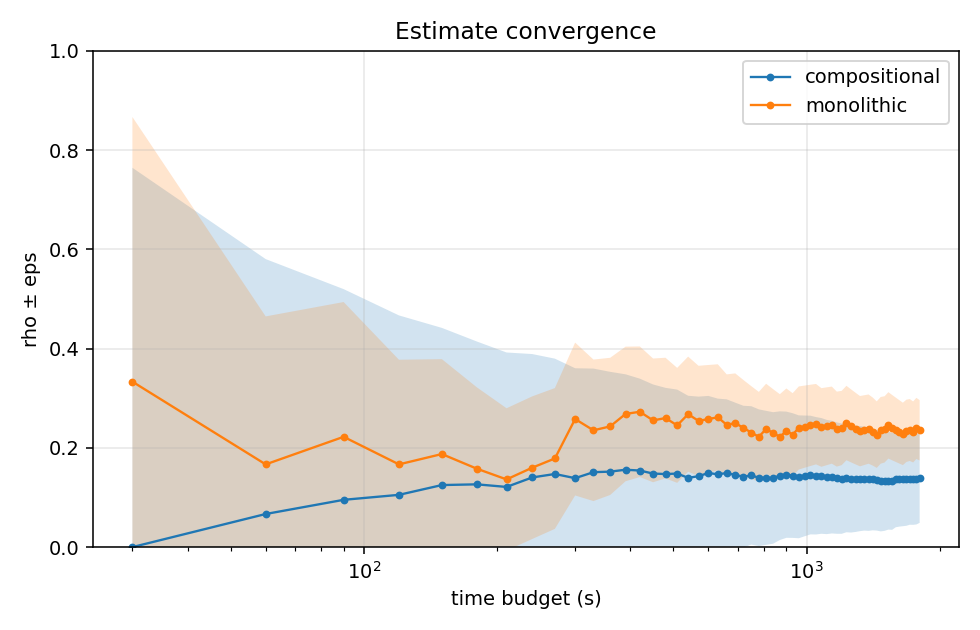
\includegraphics[width=0.49\linewidth,height=100pt,keepaspectratio]{figures/time-budget/scenic__sustained_steer__choose.png}}
    \hfill%
  \subfloat[S\,$\to$\,shuffle(C,X,O) (Scenic)]{%
       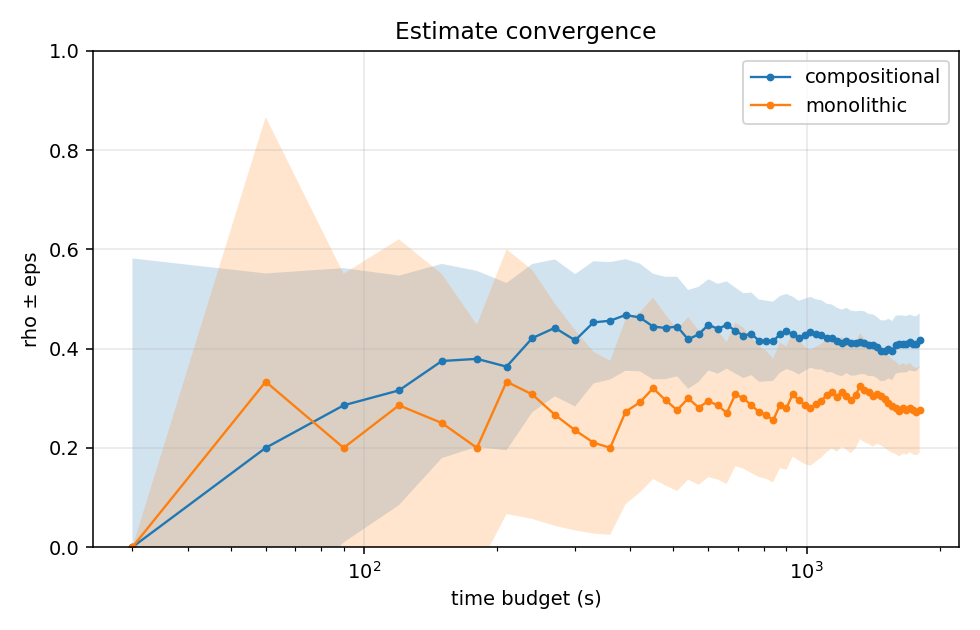
\includegraphics[width=0.49\linewidth,height=100pt,keepaspectratio]{figures/time-budget/scenic__sustained_steer__shuffle.png}}
  \caption{Fixed-time-budget results for \emph{Sustained} steering on the remaining six scenarios.}
  \label{fig:app_time_sustained}
\end{figure}
